\section{Zielsetzung}
\label{sec:Zielsetzung}
Ziel dieses Versuches ist es, den Elastizitätsmodul eines quadratischen Aluminiumstabes und eines runden Messingstabes zu bestimmen und mit Literaturwerten zu vergleichen.
\section{Theorie}
\label{sec:Theorie}
Eine Kraft, die auf eine Flächeneinheit eines Körpers wirkt, kann bei diesem eine Volumenänderung hervorrufen.
Die Komponente dieser Kraft, die orthogonal zur Oberfläche des Versuchskörpers steht, wird als Normalspannung $\sigma$ des Flächenelements bezeichnet.
Diese Spannung wird durch das Hooke´sche Gesetz:
\begin{equation}
    \sigma = E\frac{\symup{\Delta}L}{L}
\end{equation}
beschrieben. Dabei ist E der Elastizitätsmodul, welcher eine materialabhängige Konstante ist, und $\frac{\symup{\Delta}L}{L}$
die relative Änderung von $L$ einer linearen Körperdimension. Um den Elastizitätsmodul aus dieser relativen Änderung, welche zumeist sehr klein ist, zu bestimmen,
muss diese sehr präzise gemessen werden, wozu nicht immer die Geräte zur Verfügung stehen. Daher wird für diesen Versuch die Auslenkung $D$ aus einer Ruhelage
für die Messung verwendet, da diese bereits bei kleineren Kräften entsteht. Die Messverfahren dieser Größe werden in \autoref{sec:Durchführung} beschrieben.
\subsection{Biegung bei einseitiger Einspannung}
\label{subsec:EinseitigeEinspannung}
Die in \autoref{sec:Theorie} erwähnte Auslenkung $D$ ist nicht über den gesamten Querschnitt $Q$ des Stabes konstant,
sondern variiert. Daher wird die Verschiebung eines Punktes der Oberfläche an der Stelle $x$ des Stabes zur Ruhelage, wie in \autoref{fig:StabBiegung}
als $D(x)$ gemessen.
\begin{figure}[H]
    \centering
    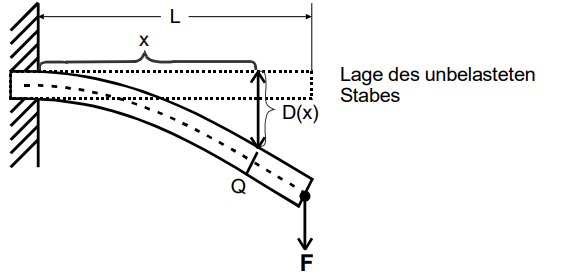
\includegraphics[scale=1]{content/StabBiegung.png}
    \caption{Einseitige Einspannung}
    \label{fig:StabBiegung}
\end{figure}
Wirkt nun eine Kraft $F$ wie in \autoref{fig:StabBiegung} auf den Stab, bewirkt diese unterhalb der in \autoref{fig:StabBiegung}
gestrichelt eingezeichneten neutralen Faser, auf der keine Spannung auftritt, Druckspannungen und oberhalb Zugspannungen.
Das Anwenden der Kraft erzeugt außerdem ein äußeres Drehmoment $M_F$. Da die eben erwähnten Zug- und Druckspannungen entgegengesetzt gleich
sind, bewirken diese auch ein Drehmoment $M_{\sigma}$, wie in \autoref{fig:InnerStab} illustriert ist.
\begin{figure}[H]
    \centering
    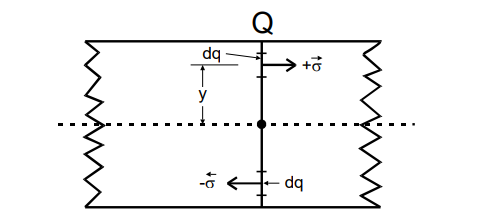
\includegraphics[scale=1]{content/InnerStab.png}
    \caption{Einseitige Einspannung}
    \label{fig:InnerStab}
\end{figure}
Dieses lässt sich nach
\begin{equation}
    \label{eqn:MSigma}
    M_{\sigma} = \int_Q y\sigma(y)dq
\end{equation}
berechnen. Die Deformation des Stabes endet, wenn sich ein Gleichgewicht zwischen den Drehmomenten 
einstellt:
\begin{equation}
    \label{eqn:MGleich}
    M_F = M_{\sigma}.
\end{equation}
Der Betrag des äußere Drehmoments $M_F$ ist hier über den Hebelarm $L-x$ definiert:
\begin{equation}
    \label{eqn:MF}
    M_F = F(L-x).
\end{equation}
Um nun den Elastizitätsmodul bestimmen zu können, wird die Beziehung zwischen Normalspannung und der Auslenkung $D$ benötigt,
welche sich zu:
\begin{equation}
    \label{eqn:SigNormD}
    \sigma = Ey\frac{d^2D}{dx^2}
\end{equation}
ergibt. Aus \eqref{eqn:SigNormD}, \eqref{eqn:MSigma}, \eqref{eqn:MF} und dem Gleichgewicht der Momente nach \eqref{eqn:MGleich} folgt:
\begin{equation}
    E\frac{d^2D}{dx^2} \int_Q y^2dq = F(L-x).
\end{equation}
Woraus sich der Ausdruck:
\begin{equation}
    I = \int_Q y^2dq(y),
\end{equation}
welcher als Flächenträgheitsmoment bezeichet wird, ergibt.
Die Auslenkung $D$ des Stabes an einer Stelle $x$ kann dann nach der folgenden Formel berechnet werden:
\begin{equation}
    \label{eqn:DvonX}
    D\left(x\right) = \frac{F}{2EI}\left(Lx^2-\frac{x^3}{3}\right),\quad 0\leq x \leq L.
\end{equation}
\subsection{Biegung bei beidseitiger Auflage}
\label{subsec:BeidseitigeAuflage}
\begin{figure}[H]
    \centering
    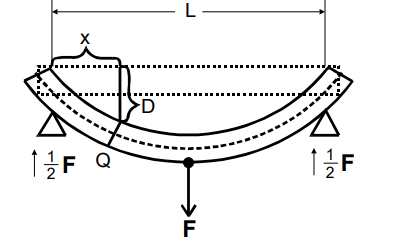
\includegraphics[scale=1]{content/StabBeidBieg.png}
    \caption{Beidseitige Auflage}
    \label{fig:StabBeid}
\end{figure}
Bei dem Wirken einer Kraft wie in \autoref{fig:StabBeid} auf einen beidseitig aufgelegten Stab ergeben sich zwei neue Drehmomente:
\begin{align}
    M_F &= -\frac{F}{2}x, &0 \leq x \leq \frac{L}{2}\\
    M_F &= -\frac{F}{2}(L-x), &\frac{L}{2} \leq x \leq L.
\end{align}
Damit folgt für die Auslenkung $D(x)$ der linken Stabhälfte:
\begin{equation}
    D(x) = \frac{F}{48EI}\left(3L^2x-4x^3\right), \quad 0 \leq x \leq \frac{L}{2}
\end{equation}
und für die rechte Stabhälfte:
\begin{equation}
    D(x) = \frac{F}{48EI}\left(4x^3 - 12Lx^2 + 9L^2x - L^3\right), \quad \frac{L}{2} \leq x \leq L.
\end{equation}

